\documentclass[12pt]{article}
\usepackage{geometry}
\usepackage{titlesec}
\usepackage{enumitem}
\usepackage{hyperref}
\usepackage{graphicx}
\usepackage{todonotes}
\usepackage{float}
\usepackage{amsmath}
\usepackage{tikz}
\usepackage{booktabs}
\usepackage{nameref}
\usepackage{url}
\usepackage{hyperref}
\usetikzlibrary{positioning, shapes.geometric, arrows.meta}

\geometry{a4paper, margin=1in}
\titleformat{\section}{\large\bfseries}{\thesection}{1em}{}
\titleformat{\subsection}{\normalsize\bfseries}{\thesubsection}{1em}{}

%-------------Ttitle Page-------------
\begin{document}

\begin{titlepage}
    \centering
    \vspace*{\fill}

    {\LARGE \textbf{Final Year Project: Preliminary Report}}\\[2em]
    {\large Development of an Explainable Deep Learning Model for}\\[0.5em]
    {\large Early Breast Cancer Detection in Singaporean Women with Dense Tissue}\\[4em]

    {\large \textbf{Justin Lim}}\\[1em]
    {\large \today}

    \vspace*{\fill}
\end{titlepage}
\newpage
\tableofcontents
\newpage

%-------------Introduction Page-------------
\newpage
\section{Introduction}
\label{chapter1}
\noindent\textbf{Word count:} 666
\vspace{1em}

\subsection{Project Template}
3.2 Project Idea 2: Deep Learning Breast Cancer Detection

\subsection{Background}

Breast cancer remains the most common cancer among women in Singapore~\cite{10}, accounting for approximately 29.6\% of all female cancers diagnosed between 2018 and 2022. The lifetime risk of developing breast cancer by age 75 is 1 in 12 women~\cite{10}. Early detection plays a critical role in improving survival outcomes, with five-year age-standardised relative survival (ASRS) improving from 49.9\% in the 1970s to 83.1\% in recent years~\cite{10}.

Despite the availability of population-wide screening initiatives such as BreastScreen Singapore~\cite{6}, several persistent challenges continue to limit the effectiveness of such programs. These include under-screening in older women, lower participation among specific ethnic groups, and diagnostic difficulties associated with dense breast tissue. Notably, women over 80 have a five-year survival rate of only 38.6\%, compared to 71.9\% for those aged 50--59~\cite{10}. 

Traditional risk models often underperform in these high-risk populations, leading to delayed or missed diagnoses. Furthermore, the interpretation of dense mammograms remains a significant clinical challenge, even for experienced radiologists. 

\subsection{Motivation}
Deep learning models particularly Convolutional Neural Networks (CNNs)—have shown significant promise in enhancing medical image interpretation, including breast cancer detection. Multiple studies have demonstrated their ability to outperform traditional statistical and risk based models, particularly in challenging scenarios such as high breast density~\cite{1,7,13}. 

Moreover, clinical adoption remains limited due to the ``black-box'' nature of deep learning models. Trust is a key barrier clinicians are unlikely to rely on algorithmic outputs without transparent decision making. Explainable AI techniques like Gradient weighted Class Activation Mapping (Grad-CAM)~\cite{5} address this challenge by offering visual explanations of model decisions. These heatmaps show which regions of an image contributed most to the model's prediction, enabling radiologists and clinicians to verify AI-generated insights.

This project is therefore motivated by two key needs: (1) to improve breast cancer detection in under screened, high risk Singaporean women using localized AI models; and (2) to enhance trust and usability in clinical workflows through model explainability.

\subsection{Project Concept}
This project proposes an \textbf{explainable deep learning system} for the classification of mammography and histopathology images to assist in breast cancer diagnosis. The system is designed to address local screening gaps by focusing on high risk features such as dense breast tissue and older age profiles.

The core of the system is a CNN based model (e.g., ResNet~\cite{17} or EfficientNet), trained to classify input images into benign or malignant categories. It will be developed using publicly available datasets, preprocessed and adapted to reflect local imaging characteristics.

To promote transparency, the system incorporates \textbf{Grad-CAM}~\cite{5} as a post hoc interpretability tool. This technique will generate heatmaps over input images, highlighting areas most influential in the model’s predictions. These visual explanations are crucial for ``human-in-the-loop'' workflows, where clinicians can evaluate and validate AI assisted diagnostics. In practice, this supports both improved diagnosis and user confidence in the tool.

\subsection{Project Objectives}
\label{sec:objectives}
The key objectives of this project are:
\begin{itemize}
    \item {Model Accuracy:} To develop a CNN-based image classification model that achieves at least {85\% accuracy} in detecting breast cancer from mammography and histopathology images.
    \item {Robustness on Local Profiles:} To ensure robust performance, particularly in {dense breast tissue and older age groups}, by maintaining {sensitivity above 80\%} across those subgroups, reflective of Singaporean demographics.
    \item {Visual Explainability Integration:} To implement {Grad-CAM visualizations} across all test predictions, integrating them into the diagnostic output to support interpretability and enable verification of the model’s focus during classification.
\end{itemize}

\subsection{Deliverables}
This project will produce the following deliverables:
\begin{itemize}
    \item {Trained CNN Model:} A fully trained and validated deep learning classification model (e.g., ResNet or EfficientNet) capable of classifying mammography and histopathology images.
    \item {Grad-CAM Visualizations:} A set of Grad-CAM heatmaps overlaid on test images to illustrate model attention and provide interpretability.
    \item {Performance Report:} A formal evaluation report detailing key classification metrics—{Accuracy, Sensitivity, Specificity, and F1-Score} across both general test sets and specific high-risk subsets.
\end{itemize}
\newpage

%-------------Literature Review Page-------------
\newpage
\section{Literature Review}
\label{chapter2}
\noindent\textbf{Word count:} 2151
\vspace{2em}

This chapter reviews the limitations of traditional breast cancer risk models, the role of deep learning in diagnostic imaging, the importance of explainability, and challenges in generalizing models across diverse populations. Each section provides justification for the design choices and objectives outlined in this project emphasizing the need for a localized, explainable deep learning system in Singapore's screening context.

\subsection{Analysis of Similar Projects and Tools}

To ensure the proposed system is both technically sound and contextually relevant, it is important to review recent advancements in AI-assisted breast cancer screening. This comparative analysis highlights key successes and limitations of existing tools and research. By examining how these systems were designed, evaluated, and applied in real-world scenarios, this can identify best practices and avoid common pitfalls. This analysis also helps justify the architectural and design decisions made in this project particularly the emphasis on explainability, local adaptation, and clinician-in-the-loop deployment.

\begin{itemize}
    \item \textbf{Google Health / DeepMind – Mammogram AI System} \\
    This system, trained on over 90{,}000 mammograms, demonstrated strong diagnostic capabilities, outperforming radiologists in controlled trials~\cite{11}. However, the system's performance decreased significantly when applied to external datasets, highlighting its limited generalization capabilities. To mitigate such risks, this project incorporates stratified testing and local data simulation techniques to better represent the breast density profiles and demographic variations seen in Singapore.

    \item \textbf{Zebra Medical Vision – Scalable Cancer Detection Tools} \\
    Zebra’s AI tools gained traction due to their regulatory approval and ease of integration into existing cloud-based radiology systems~\cite{12}. While their deployment model is highly scalable, a lack of interpretability in model decisions has raised concerns about trust and transparency. To address this, the proposed system integrates Grad-CAM visualizations directly into the diagnostic output, ensuring interpretability without sacrificing operational compatibility.

    \item \textbf{Shen et al. (2019) – CNN-Based Mammogram Classifier} \\
    Shen et al. applied CNNs to mammographic image classification with encouraging results~\cite{7}, yet their work revealed an ongoing reliance on large, high-quality, annotated datasets for training. Given the challenges of acquiring such datasets locally, this project includes data augmentation techniques and a compact network architecture to maintain performance while coping with limited annotated image availability in Singapore.
\end{itemize}

\noindent \textbf{Summary of Insights and Application:} \\
From these projects, several key insights emerge: the importance of robust validation across diverse populations, the need for transparent model outputs, and the value of seamless integration into clinical workflows. These findings shape this project’s approach by ensuring the model is both interpretable (via Grad-CAM) and tuned to local breast density distributions. Furthermore, clinician-in-the-loop design is adopted to foster trust, prevent overreliance on automation, and ensure that AI predictions enhance rather than override expert judgment. By incorporating these lessons, the proposed prototype aims to strike a balance between technical performance, clinical usability, and ethical responsibility.

\subsection{Role of Deep Learning in Breast Cancer Imaging}

To justify the deep learning approach used in this project, it is essential to examine how convolutional neural networks (CNNs) have enhanced breast cancer diagnostics. Unlike traditional models that rely on structured variables such as age and family history, CNNs operate directly on full field mammograms. This enables them to detect complex spatial features such as tissue asymmetry, mass shape, and density patterns that often precede clinical symptoms. These characteristics are particularly critical in screening contexts involving dense breast tissue, a trait common among women in Singapore~\cite{6}.

Evidence from Yala et al.~\cite{1} offers strong justification for the adoption of CNN-based image analysis as the foundation of this project. In their study, three models were compared: the Tyrer-Cuzick clinical risk model, a CNN-based image-only model, and a hybrid model combining clinical and imaging features. Both deep learning models outperformed the traditional approach, with the hybrid model achieving the highest detection rates especially among patients with dense breast tissue. Appendix Figure~\ref{fig:hybrid_density} demonstrates that these CNN-driven models captured significantly more cancers in high-risk, dense-tissue populations. This highlights the advantage of CNNs in extracting detailed visual patterns and supports their role as the core architecture for this project’s predictive pipeline.

Moreover, the hybrid model in Yala et al.~\cite{1} which combines image features with clinical metadata demonstrated marginal performance improvements over the image only CNN. For this project, this suggests that integrating additional patient specific factors (e.g., breast density or age) into the pipeline could enhance model calibration for local populations. This aligns with the desired outcome of increasing detection performance specifically in Singaporean women, where dense tissue and age related diagnostic delays are prevalent~\cite{6,10}.

Shen et al.~\cite{7} further reinforce this direction by showcasing the use of CNNs in generating Grad-CAM-based heatmaps that highlight diagnostically salient regions within mammograms. These visualizations not only aid radiologists in understanding the rationale behind predictions but also reduce overreliance on black-box outputs. As illustrated in their study, Grad-CAM helped improve trust in AI assisted diagnostics by revealing consistent and clinically relevant attention areas. This motivates the project's focus on incorporating visual explainability as an interpretability layer over CNN predictions, ultimately supporting clinician adoption.

Taken together, these works justify the technical foundations of this project: selecting CNN-based models for their spatial learning capacity, exploring hybrid architectures for incremental performance gain, and embedding explainability to facilitate clinical acceptance in the Singaporean screening context~\cite{1,6,7}.

\subsection{Role of Deep Learning in Breast Cancer Imaging}

To justify the deep learning approach used in this project, it is essential to examine how convolutional neural networks (CNNs) have enhanced breast cancer diagnostics. Unlike traditional models that rely on structured variables such as age and family history, CNNs operate directly on full field mammograms. This enables them to detect complex spatial features like tissue asymmetry, mass shape, and density patterns that often precede clinical symptoms especially critical in dense breast tissue, a trait common among women in Singapore~\cite{6}.

Evidence from Yala et al.~\cite{1} offers strong justification for adopting CNN-based image analysis. In their study, three models were compared: the Tyrer-Cuzick clinical risk model, a CNN-based image-only model, and a hybrid model combining clinical and imaging features. Both deep learning models outperformed the traditional approach, with the hybrid achieving the highest detection rates especially among patients with dense breast tissue. Appendix Figure~\ref{fig:hybrid_density} shows that CNN-driven models captured significantly more cancers in high-risk, dense-tissue populations, supporting their role as the core architecture for this project’s predictive pipeline.

Moreover, the hybrid model in Yala et al.~\cite{1} showed only marginal improvements over the image-only CNN. For this project, this suggests integrating patient-specific factors (e.g., breast density or age) could enhance model calibration for local populations. This aligns with the goal of improving detection in Singaporean women, where dense tissue and age-related diagnostic delays are prevalent~\cite{6,10}.

Shen et al.~\cite{7} reinforce this direction by showcasing CNNs with Grad-CAM, which highlight diagnostically salient regions. These visualizations help radiologists understand the model’s rationale, improving trust in AI-assisted diagnostics. This motivates the project’s focus on embedding explainability into its pipeline.

Taken together, these works justify the project’s technical foundations: selecting CNN-based models for spatial learning, exploring hybrid architectures for incremental performance gain, and embedding explainability to support clinical acceptance in Singapore~\cite{1,6,7}.

\subsection{Explainability in Medical AI}

While deep learning (DL) models have achieved strong performance in medical imaging, their “black box” nature remains a barrier to clinical adoption. Unlike traditional models with defined features, CNNs often produce predictions without transparent reasoning. In high-stakes domains like cancer diagnosis, this lack of interpretability raises ethical and practical concerns especially when errors could cause misdiagnosis or delayed treatment~\cite{3}.

This issue is especially relevant to this project, which targets breast cancer screening in Singapore. Clinicians need to understand how and why a model makes a prediction to trust and act on it. As Ching et al.~\cite{3} emphasize, explainability is not just a technical add-on but a prerequisite for responsible AI use in healthcare.

To overcome this limitation, the project incorporates Gradient-weighted Class Activation Mapping (Grad-CAM) into its CNN architecture. Grad-CAM generates heatmaps showing which mammogram regions most influenced a prediction. These explanations help radiologists validate whether the model focuses on clinically relevant structures like calcifications or asymmetries~\cite{5}.

Selvaraju et al.~\cite{5} demonstrated how Grad-CAM highlights malignancy-related areas in medical images. Appendix Figure~\ref{fig:gradcam} shows a representative output where red activation zones align with tumor like regions. This supports the project’s goal of clinician-aligned AI: when a model’s attention corresponds to known diagnostic features, trust increases. Conversely, if attention maps focus on irrelevant regions, it may indicate model failure and justify retraining~\cite{5}.

This is especially important in Singapore, where diverse ethnic backgrounds and diagnostic baselines vary~\cite{6}. Explainable models offer a shared visual rationale for predictions and reduce automation bias by keeping radiologists in the loop~\cite{3}.

Moreover, Grad-CAM integration enables routine auditing and case review. Heatmaps can be stored and monitored over time supporting traceability and aligning with the Ministry of Health’s emphasis on accountability~\cite{6}.

In summary, explainability is central to the viability of AI in breast cancer screening. By embedding Grad-CAM, this project ensures predictions are accurate, interpretable, and clinically actionable~\cite{5}.

subsection{Dataset Diversity and Generalization}

A major consideration when designing AI systems for breast cancer screening is generalizability. Many deep learning models are trained on Western datasets~\cite{1}, which differ in clinical practices, imaging protocols, and demographics from Southeast Asia.

This issue is particularly relevant to Singapore. Chau et al.~\cite{6} found that Singaporean women often have denser breast tissue and are diagnosed at younger ages. Dense tissue increases cancer risk and reduces mammography effectiveness, raising false negative rates. Cultural factors like screening hesitancy further complicate this. These traits highlight the importance of developing models aligned with local characteristics.

Yala et al.~\cite{1} achieved strong results on U.S. data using a hybrid model of image and clinical features, but its effectiveness in Singapore is uncertain. Appendix Figure~\ref{fig:hybrid_density} shows cancer incidence varies significantly by tissue density and risk category. While image-driven models show promise, local calibration is needed for relevance.

This is reinforced by Raghu et al.~\cite{2}, who found that ImageNet pretraining provides little benefit in medical imaging. Appendix Figure~\ref{fig:lit2table7} supports this, motivating the project’s use of a lightweight CNN trained on domain-specific mammography data.

Another barrier is dataset scarcity. In Singapore, access to annotated medical data is limited due to privacy and cohort size. Cheplygina et al.~\cite{4} suggest methods like semi-supervised learning (SSL), weak supervision, and multi-instance learning (MIL) to mitigate this. These approaches reduce the need for extensive labeling and are more feasible in data-constrained environments.

This project adopts several such strategies: dense tissue variability is simulated through augmentation; focal loss addresses malignancy underrepresentation~\cite{2}; and the architecture is built for future fine-tuning on local data. These steps ensure clinical relevance, demographic alignment, and adaptability.

In summary, generalization cannot be assumed. By emphasizing localization, data-efficient learning, and domain-specific training, this project supports a clinically aligned breast cancer screening solution for Singapore.

\subsection{Summary of Gaps and Relevance}

The literature highlights several critical gaps that this project directly addresses. Existing clinical models lack sensitivity in dense breast tissue~\cite{1}, most deep learning models are trained on non-local datasets~\cite{6}, and explainability remains a major barrier to clinical trust~\cite{3,5}. To respond, this project adopts a CNN pipeline with Grad-CAM overlays, simulates dense tissue cases through augmentation, and emphasizes transparency and localization to enhance both performance and clinical relevance in Singapore’s screening context.

\begin{itemize}
\item \textbf{Poor Sensitivity in Dense Breast Tissue}\
Clinical risk models like Gail and Tyrer-Cuzick overlook visual patterns in mammograms and perform poorly in women with dense breasts—a common trait among Singaporean women~\cite{6}. Deep learning offers superior image-based prediction~\cite{1,7}. This project builds a CNN trained on full-field mammograms to capture high-resolution diagnostic features and improve sensitivity in underrepresented tissue types.

\item \textbf{Lack of Explainability Reduces Clinical Adoption}\\
CNN models are often criticized for their "black-box" nature~\cite{3,5}, limiting their adoption in clinical settings. Grad-CAM provides visual explanations by highlighting regions that drive predictions~\cite{5}. This project embeds Grad-CAM into the diagnostic pipeline to support radiologist trust, human oversight, and accountable decision-making.

\item \textbf{Limited Generalization from Western-Centric Datasets}\\
Most AI models are developed using Western cohorts, which differ in breast density, screening behavior, and risk profiles~\cite{6}. This project introduces region-specific augmentations and stratified evaluations to simulate local conditions, increasing generalizability to Singaporean populations.
\end{itemize}

\vspace{0.5em}
Collectively, these gaps justify the core architecture of this project:
\begin{itemize}
    \item CNN-based image models are prioritized over questionnaire-based tools for precision screening;
    \item Grad-CAM explainability ensures clinical interpretability and user trust;
    \item Training pipelines are adapted to local demographic factors;
    \item Lightweight architectures and weak supervision accommodate Singapore's data limitations;
    \item Transfer learning is validated critically rather than assumed.
\end{itemize}

These strategies form the foundation of a culturally responsive, explainable AI pipeline optimized for breast cancer screening in Singapore.


%-------------Project Design Page-------------
\newpage
\section{Project Design}
\label{chapter3}
\noindent\textbf{Word count:} 1881
\vspace{1em}

\subsection{User and Domain Context}
This project targets clinical radiologists and public health administrators within Singapore’s national breast cancer screening infrastructure. It focuses on AI-assisted diagnostic tools for mammogram analysis, especially for women aged 40–60 with dense breast tissue a demographic underrepresented in most Western datasets, necessitating a localized system.

These users are directly involved in interpreting screening results and making early intervention decisions. A tailored AI tool can improve diagnostic accuracy, reduce workload, and support informed public health strategies, especially in populations with unique imaging challenges like dense tissue.

\subsection{System Architecture}

Figure~\ref{fig:system_architecture} shows the architecture of the proposed breast cancer risk prediction system, covering image preprocessing, CNN-based classification, and explainability via Grad-CAM~\cite{1,5}. Presenting the architecture upfront anchors the subsequent module descriptions.

The pipeline starts with mammographic images, which go through preprocessing (see Section~3.4) involving grayscale conversion, normalization, and augmentation. These standardized images are then fed into a CNN backbone (e.g., ResNet-50 or EfficientNet-B0) for feature extraction.


From here, the architecture diverges into two parallel outputs:
\begin{itemize}
    \item A prediction head that computes a cancer risk probability score (detailed in the model section).
    \item A Grad-CAM explainability module that generates visual heatmaps to highlight important diagnostic regions.
\end{itemize}

\begin{figure}[H]
    \centering
    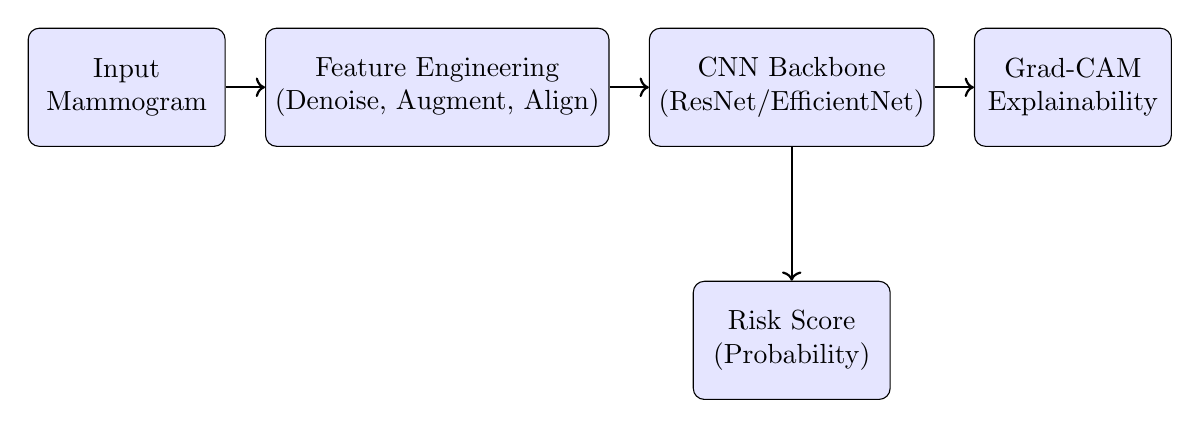
\begin{tikzpicture}[
        node distance=1cm and .5cm,
        box/.style={rectangle, draw=black, fill=blue!10, rounded corners, minimum width=2.5cm, minimum height=1.5cm, align=center},
        arrow/.style={->, thick}
        ]
        
        \node[box] (input) {Input\\Mammogram};
        \node[box, right=of input] (featureeng) {Feature Engineering\\(Denoise, Augment, Align)};
        \node[box, right=of featureeng] (cnn) {CNN Backbone\\(ResNet/EfficientNet)};
        \node[box, right=of cnn] (gradcam) {Grad-CAM\\Explainability};
        \node[box, below=1.7cm of cnn] (output) {Risk Score\\(Probability)};
        
        \draw[arrow] (input) -- (featureeng);
        \draw[arrow] (featureeng) -- (cnn);
        \draw[arrow] (cnn) -- (gradcam);
        \draw[arrow] (cnn) -- (output);
    \end{tikzpicture}
    \caption{System architecture for explainable breast cancer risk prediction using convolutional neural networks (CNNs)~\cite{1} and Grad-CAM~\cite{5}, with feature engineering integrated as a preprocessing stage.}
    \label{fig:system_architecture}
\end{figure}

\paragraph{Input Preprocessing Layer.}

To ensure model robustness, this stage standardizes image inputs for consistent downstream processing. Based on best practices in mammogram preprocessing~\cite{7,14}, and observations from the DDSM dataset~\cite{17}, the following steps are included:

\begin{itemize}
    \item {Grayscale conversion:} Images are converted to 8-bit grayscale to reduce computational complexity while preserving critical tissue structures.
    \item {Histogram normalization:} Applied to minimize contrast variability across acquisition devices, aiding generalization.
    \item {Resizing:} Images are resized to 224x224 pixels to match CNN input requirements~\cite{1}, enabling model reuse and compatibility.
    \item {ROI extraction:} Regions of interest are isolated by removing annotations and borders, preventing irrelevant artifacts from biasing the model.
\end{itemize}
\paragraph{CNN Backbone.}
Feature extraction is handled by ResNet-50 or EfficientNet-B0, selected for their proven performance in medical imaging~\cite{1,7}. ResNet offers accuracy and depth, while EfficientNet provides computational efficiency through compound scaling.

\paragraph{Prediction Head.}
Extracted features are passed through fully connected layers, ending in a sigmoid neuron that outputs a cancer risk probability score. Binary cross-entropy is the default loss, with optional focal loss~\cite{2} to improve sensitivity to rare malignancies and address class imbalance.

\paragraph{Explainability Module.}
To enhance transparency, Grad-CAM~\cite{5} highlights input regions that influenced predictions. This supports clinical trust, especially in dense or ambiguous cases. Figure~\ref{fig:system_architecture} shows how the CNN output feeds both the risk score and the Grad-CAM branch.

\paragraph{Design Considerations.}
Modules are kept modular for future upgrades—such as fine-tuning on Singapore-specific data, adding metadata, or supporting multi-view inputs~\cite{8}. This ensures adaptability to evolving datasets and deployment needs, balancing predictive performance with clinical usability.

\subsection{Dataset Used}

The model is trained and evaluated using the CBIS-DDSM dataset from Kaggle~\cite{cbis_ddsm_kaggle}, selected for its accessibility and preprocessing.

\paragraph{Primary Dataset – DDSM.}
The DDSM~\cite{17} contains over 2,600 cases, each with four standard views and pathology-verified annotations. Its volume and case diversity support robust CNN training and classification of both benign and malignant samples.

\paragraph{Auxiliary Dataset – BreaKHis.}
The BreaKHis dataset~\cite{18}, though not used in this prototype, offers cellular-level detail valuable for future domain adaptation studies between mammography and histopathology.

\paragraph{Singapore-Specific Contextualization.}
To reflect local screening challenges, future versions may incorporate traits from the Singapore Breast Cancer Cohort~\cite{6} and BreastScreen Singapore~\cite{19}, including dense breast tissue prevalence and smaller breast volumes. Synthetic augmentation is used to simulate these traits in the current prototype.

\subsection{Feature Engineering}
\label{subsection:Feature Engineering}

As indicated in the System Architecture (Figure~\ref{fig:system_architecture}), feature engineering is a foundational component of the preprocessing module. It ensures that raw mammographic data are transformed into a consistent and clinically enriched format suitable for CNN-based analysis. This step precedes the CNN backbone in the pipeline and directly influences both the prediction accuracy and the quality of Grad-CAM visualizations.

Figure~\ref{fig:end_to_end_pipeline} expands on this preprocessing phase in greater detail illustrating the specific transformations applied to raw DICOM images before they are passed into the CNN for feature extraction and classification.

\begin{figure}[H]
    \centering
    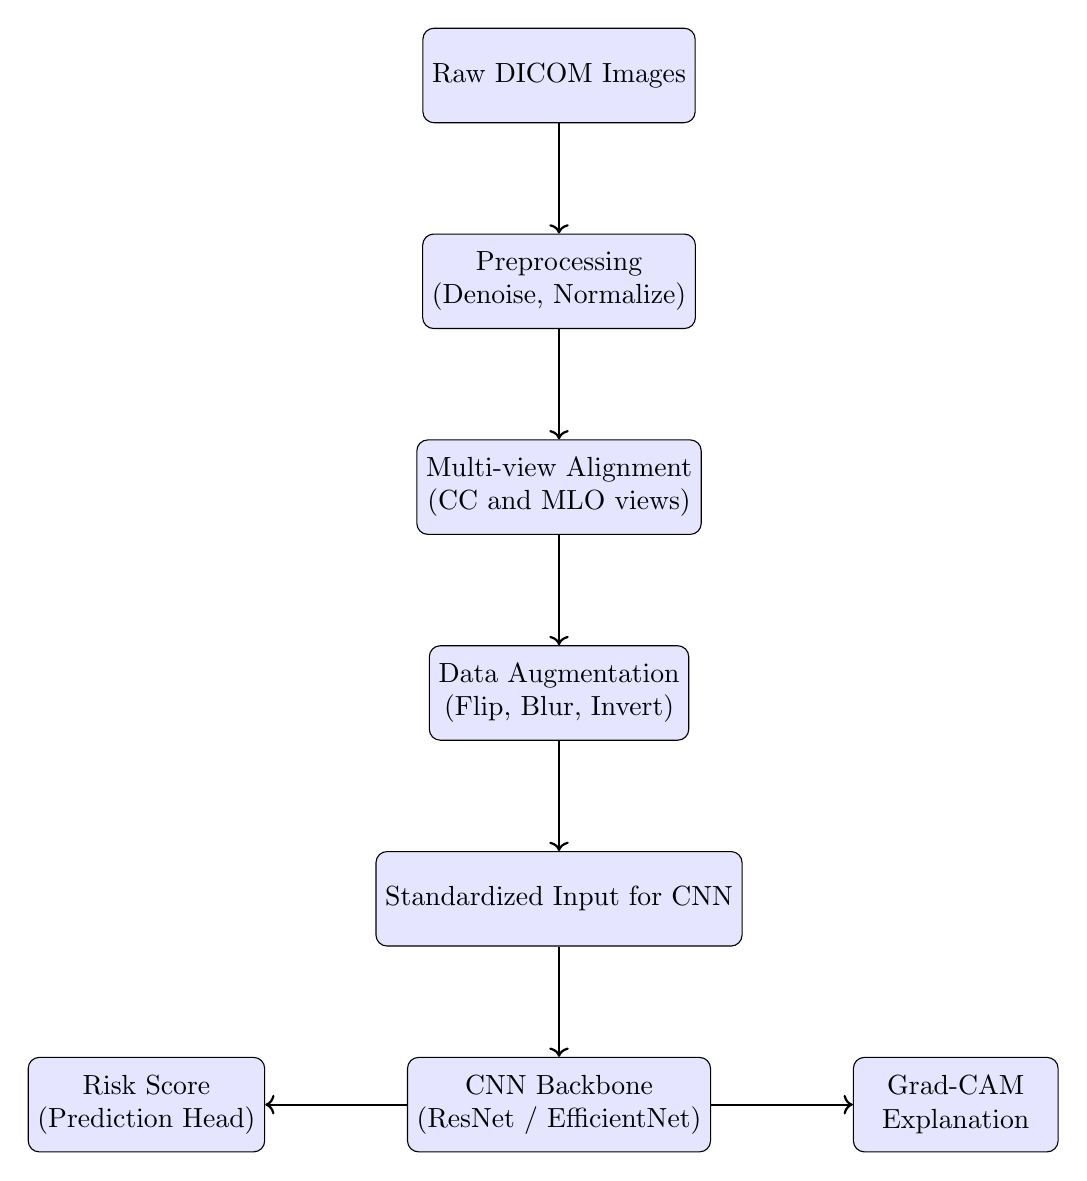
\begin{tikzpicture}[
        node distance=1.4cm and 0.8cm,
        box/.style={rectangle, draw=black, fill=blue!10, rounded corners, minimum width=2.6cm, minimum height=1.2cm, align=center},
        arrow/.style={->, thick}
        ]
        
        \node[box] (dicom) {Raw DICOM Images};
        \node[box, below=of dicom] (preprocess) {Preprocessing\\(Denoise, Normalize)};
        \node[box, below=of preprocess] (align) {Multi-view Alignment\\(CC and MLO views)};
        \node[box, below=of align] (augment) {Data Augmentation\\(Flip, Blur, Invert)};
        \node[box, below=of augment] (standard) {Standardized Input for CNN};
        \node[box, below=of standard] (cnn) {CNN Backbone\\(ResNet / EfficientNet)};
        \node[box, right=1.8cm of cnn] (gradcam) {Grad-CAM\\Explanation};
        \node[box, left=1.8cm of cnn] (score) {Risk Score\\(Prediction Head)};

        \draw[arrow] (dicom) -- (preprocess);
        \draw[arrow] (preprocess) -- (align);
        \draw[arrow] (align) -- (augment);
        \draw[arrow] (augment) -- (standard);
        \draw[arrow] (standard) -- (cnn);
        \draw[arrow] (cnn) -- (gradcam);
        \draw[arrow] (cnn) -- (score);
    \end{tikzpicture}
    \caption{End-to-end pipeline for breast cancer risk prediction, integrating preprocessing, multi-view feature alignment, CNN classification, and visual explainability.}
    \label{fig:end_to_end_pipeline}
\end{figure}

The purpose of this step is to enhance generalization and sensitivity, particularly in dense breast tissue scenarios that are common among Singaporean women. It includes denoising, contrast enhancement, multi-view alignment, and augmentation strategies all of which standardize input images and simulate clinical variability. 

\paragraph{Preprocessing and Augmentation.}
The initial phase of feature engineering focuses on cleaning and enhancing the diagnostic quality of raw mammograms. This step is essential to ensure consistent model input and eliminate irrelevant imaging artifacts.

\begin{itemize}
    \item \textbf{Denoising:} Median filtering removes impulse noise (e.g., salt-and-pepper artifacts) while preserving fine structural detail important for detecting subtle anomalies like microcalcifications.
    \item \textbf{Contrast enhancement:} CLAHE (contrast-limited adaptive histogram equalization)~\cite{14} enhances local contrast, improving visibility of faint lesions, especially in dense tissue environments.
    \item \textbf{Normalization:} Pixel values are rescaled to $[0,1]$ or z-normalized to ensure uniform dynamic range, enabling more stable model convergence.
\end{itemize}

After standardization, augmentation techniques are applied to increase data diversity and improve model robustness:

\begin{itemize}
    \item \textbf{Geometric:} Random flipping, cropping, and small-angle rotations ($\pm15^{\circ}$) simulate positioning variability during imaging.
    \item \textbf{Photometric:} Gaussian blurring and contrast jitter mimic scanner inconsistencies and imaging noise.
    \item \textbf{Semantic:} Intensity inversion introduces exposure variation and histogram shifts, improving cross-device generalization.
\end{itemize}

These transformations help prevent overfitting and prepare the model for deployment across heterogeneous clinical environments.

\paragraph{Multi-View Spatial Context.}
Breast screening typically involves multiple views: cranio-caudal (CC) and mediolateral oblique (MLO). Rather than treating each view independently, this project uses a multi-view strategy to leverage spatial correlations across angles. This is based on the approach by Geras et al.~\cite{8}, who showed that multi-view CNNs improve lesion localization and diagnostic accuracy.

\begin{figure}[H]
    \centering
    \includegraphics[width=0.95\textwidth]{images/GerasFig1.png}
    \caption{High-resolution mammogram processing via multi-view deep CNNs. Adapted from Geras et al.~\cite{8}.}
    \label{fig:geras}
\end{figure}

Both CC and MLO views are preprocessed and aligned to maintain anatomical consistency. This strategy enables the model to capture bilateral asymmetries, view-dependent lesion projections, and complementary diagnostic signals critical for real-world screening reliability.

\paragraph{Domain-Specific Feature Emphasis.}
In addition to automated learning, domain knowledge is embedded to focus the model on clinically meaningful features:

\begin{itemize}
    \item \textbf{Asymmetry detection:} Breast difference maps highlight abnormal structural discrepancies between left and right sides.
    \item \textbf{Texture emphasis:} Gabor filters~\cite{20} are used to visualize texture patterns—such as spiculations—that are indicative of malignancy.
    \item \textbf{Density-informed stratification:} BI-RADS (Breast Imaging Reporting and Data System)~\cite{16} density levels are approximated via grayscale histograms and used to weight loss functions, placing more emphasis on dense cases that are diagnostically challenging.
\end{itemize}

These domain-guided strategies strengthen the model’s interpretability and diagnostic sensitivity. They also support the project’s goal of building a culturally adapted, clinically grounded AI system for breast cancer risk prediction.

\subsection{Algorithm Selection}

Model architecture is chosen based on diagnostic accuracy, computational efficiency, and interpretability. ResNet-50 serves as the primary benchmark due to its success in medical imaging tasks~\cite{1,7}. 

To evaluate trade-offs, two alternatives are explored:

\begin{itemize}
    \item \textbf{EfficientNet-B0:} EfficientNet’s compound scaling achieves strong performance with fewer parameters than ResNet, making it suitable for resource-constrained environments such as hospital systems or edge devices.

    \item \textbf{Custom Shallow CNN:} Following Raghu et al.~\cite{2}, who found that transfer learning from datasets like ImageNet may offer limited benefit in medical domains, a smaller model trained from scratch is used to test performance in a localized screening context.
\end{itemize}

Benchmarking across these models helps determine the optimal trade-off between accuracy, efficiency, and generalization especially for dense tissue scenarios in Singaporean women.

\paragraph{Optimization and Regularization.}
Models are optimized using Adam with a cyclical learning rate. Dropout is applied after the final dense layer to mitigate overfitting, and early stopping (patience = 10) is used to prevent unnecessary training epochs.

\vspace{1em}

\subsection{Evaluation Metrics}

\paragraph{Quantitative Metrics.}
Performance is evaluated using metrics aligned with clinical relevance, risk stratification, and imbalanced data challenges:

\begin{itemize}
    \item \textbf{AUC (Area Under the ROC Curve):} Measures the model’s ability to distinguish between malignant and benign cases across thresholds. It is the primary metric due to its value in screening workflows~\cite{1}.
    
    \item \textbf{Sensitivity \& Specificity:} Critical in breast cancer screening. Sensitivity is prioritized to minimize false negatives, particularly in dense breast tissue cases where early-stage cancers are harder to detect~\cite{6}.
    
    \item \textbf{F1-Score:} Offers a balanced view of precision and recall, essential in imbalanced datasets where accuracy alone can be misleading.
\end{itemize}

\paragraph{Explainability Evaluation.}
Grad-CAM heatmaps are overlaid on mammograms and visually inspected where possible—by domain experts to assess alignment with diagnostic features.

\begin{figure}[H]
    \centering
    \includegraphics[width=0.8\textwidth]{images/gradcam_sample.png}
    \caption{Grad-CAM visualizations showing model attention over mammograms. Red indicates regions of high diagnostic interest.}
\end{figure}

% \paragraph{Qualitative Explainability Assessment.}
% Beyond standard performance metrics, interpretability is essential in medical imaging. Kim et al.\ (2018) proposed the Data-driven Imaging Biomarker model (DIB-MG), which generates attention maps that highlight risk-relevant regions in mammograms. Their work supports the use of Grad-CAM as a means to validate model behavior against radiological intuition. As shown in Figure~\ref{fig:kim2018}, attention maps provide visual grounding for predictions, which is key to clinical trust and regulatory validation.

% \begin{figure}[H]
%     \centering
%     \includegraphics[width=0.85\textwidth]{images/KimFig3.png}
%     \caption{DIB-MG: Attention-based imaging biomarker model localizing high-risk regions. Adapted from Kim et al.\ (2018).}
%     \label{fig:kim2018}
% \end{figure}

\paragraph{Risk Stratification.}
Patients are ranked by predicted risk scores and divided into deciles. Metrics like:
\begin{itemize}
    \item \textbf{Cumulative incidence in top decile}
    \item \textbf{Hazard ratio (HR)}
    \item \textbf{Calibration curves}
\end{itemize}
are computed to evaluate clinical utility.

\paragraph{Cross-validation.}
A 5-fold stratified cross-validation is used during training. The final model is evaluated on a held-out test set to prevent data leakage and overfitting.

\vspace{1em}

\paragraph{Conclusion.}
This project adopts a structured, explainable deep learning architecture validated through standard and custom metrics. By leveraging Grad-CAM, dense tissue-aware training, and Singapore-specific context simulation, the design aligns both technically and clinically with the needs of under-screened populations in Southeast Asia.

\subsection{Work Plan and Project Timeline}

This project follows a structured timeline spanning from July to early September 2024, divided into four main phases to manage complexity, reduce risk, and ensure timely delivery. The planning was informed by a top-down decomposition of tasks based on project requirements, module interdependencies, and key submission milestones (e.g., briefing, prototype, final report). Each phase was allocated based on task duration, estimated workload.

\begin{enumerate}
    \item \textbf{Project Conceptualising (Weeks 1–5):} This phase focuses on understanding the problem domain, reviewing prior work, and preparing early deliverables (e.g., proposal video, literature review). Front-loading research activities ensures a strong theoretical foundation for later implementation.

    \item \textbf{Project Planning and Design (Weeks 5–9):} Here, the system architecture, dataset choices, and evaluation methods are formalized. Time is also allocated for early prototyping to identify technical feasibility and refine scope before development.

    \item \textbf{Development and Testing (Weeks 10–18):} The longest phase, this includes model training, iterative testing, and evaluation. Tasks are sequenced to allow progressive model improvements while maintaining checkpoints for early validation. This modular approach reduces integration risk.

    \item \textbf{Final Sprint (Weeks 18–25):} Reserved for final evaluation, report writing, and video presentation. A buffer period is also included (Week 25) to manage unexpected delays, ensuring submission readiness without compromising quality.
\end{enumerate}

Figure~\ref{fig:gantt} presents the Gantt chart visualizing these stages. 

\begin{figure}[H]
    \centering
    \includegraphics[width=\textwidth]{images/PPR_GanttChart.png}
    \caption{Project Gantt chart showing planned activities from July to September 2024, divided into phases of research, design, development, and reporting.}
    \label{fig:gantt}
\end{figure}

%-------------Feature Prototype Page-------------
\newpage
\section{Feature Prototype}
\noindent\textbf{Word count:} 1302
\vspace{1em}

\subsection{Development Strategy}
This section documents the current implementation progress of the AI-powered breast cancer screening tool, referencing the modular pipeline and objectives described in \hyperref[chapter3]{Chapter 3} (Project Design).

The system was developed using a modular 4-stage pipeline:
\begin{enumerate}
    \item Data Preprocessing (\texttt{01\_preprocessing.ipynb})
    \item Model Training (\texttt{02\_model\_training.ipynb})
    \item Grad-CAM Visualization (\texttt{03\_gradcam\_visualization.ipynb})
    \item Evaluation (\texttt{04\_evaluation.ipynb})
\end{enumerate}

Each notebook represents a key module of the system and is accessible via the project repository: \href{https://github.com/justinlim00/FYP-Overview25/tree/main/FYP%20Project/FYP%20Project%20Code%20V1/notebooks}{GitHub repository}.

\begin{itemize}
    \item The development followed a staged strategy: preprocessing ensured standardized image dimensions and class balance, followed by a custom CNN trained with regularization and class imbalance handling. This baseline aligns with \hyperref[sec:objectives]{Objective 1 (Model Accuracy)}.
    
    \item To address \textbf{Objective 2 (Robustness)}, the system used stratified splitting and class weights to improve detection in rare cases such as malignancies and dense tissue profiles. Threshold tuning during evaluation emphasized sensitivity for early cancer detection.

    \item \textbf{Objective 3 (Explainability)} was implemented via Grad-CAM, generating heatmaps that highlight regions influencing predictions. This improves clinical interpretability and supports trust in AI-assisted workflows.
\end{itemize}

This prototype forms a complete, modular foundation. It supports future additions (e.g., transfer learning, UI integration), and identifies performance and explainability gaps that will guide the final development phase outlined in \hyperref[improvements]{Section~4.3}.

\subsection{Implemented Modules}
The system was developed in a staged, dependency-driven order to ensure a functional pipeline from the outset. Data preprocessing was prioritized to standardize inputs, followed by model training, interpretability, and finally, evaluation. This sequence aligns with the overall system architecture and the objectives outlined in \hyperref[chapter1]{Chapter 1}

\begin{enumerate}
    \item Data preprocessing must precede all modeling tasks.
    \item Training a working baseline model is a prerequisite for meaningful evaluation or comparison.
    \item Visualization tools (Grad-CAM) were developed early to ensure that model interpretability (Objective 2) could be validated in parallel with model accuracy.
\end{enumerate}

This prioritization ensures that the foundational system works end-to-end, allowing later additions (e.g., pretrained models, dashboard UI) to be integrated without reengineering the core pipeline.


\paragraph{\texttt{01\_preprocessing.ipynb}}
This module establishes the foundation for all downstream processing by ensuring input image consistency, format standardization, and class distribution balance. The CBIS-DDSM dataset~\cite{18} was used as the primary data source, containing curated digitized mammography images labeled with biopsy-confirmed pathology.

Key steps include:
\begin{itemize}
    \item \textbf{Grayscale Conversion:} All input PNG images were converted to grayscale to reduce channel redundancy, aligning with common practices in medical imaging literature~\cite{7}.
    \item \textbf{Size Standardization:} Images were resized to a fixed input shape of 224$\times$224 pixels to fit the input requirements of CNN architectures like ResNet and EfficientNet. This ensures model compatibility and allows efficient batch processing.
\end{itemize}

The preprocessing script is modular, designed for reuse across multiple experiments. It includes parameterized options to support future image augmentation operations (e.g., rotations, contrast enhancement) in later development stages.

\vspace{0.5em}

\paragraph{\texttt{02\_model\_training.ipynb}}
This module implements the core classification model using a custom Convolutional Neural Network (CNN), selected for its balance between interpretability, computational efficiency, and suitability for binary medical imaging tasks~\cite{17}.

\begin{itemize}
    \item \textbf{Model Architecture:} \\
    The model accepts $224 \times 224$ grayscale images as input. It has two convolutional blocks: the first with a Conv2D layer (32 filters, $3 \times 3$ kernel, ReLU) and MaxPooling2D; the second repeats this with 64 filters. Features are flattened and passed through a Dense layer (128 ReLU units) and Dropout (0.5). The final output is a sigmoid-activated neuron for binary classification.
    
    \item \textbf{Training Configuration:} \\
    The model uses binary cross-entropy loss and the Adam optimizer (learning rate = 0.001), with batch size 32. Early stopping (patience = 5) prevents overfitting and conserves resources.
\end{itemize}

Validation accuracy plateaued near 80\%, with divergence in later epochs suggesting overfitting prompting plans for batch normalization, learning rate tuning, and stronger augmentation.

\paragraph{Handling Class Imbalance} CBIS-DDSM shows class imbalance. To counter this, Keras’s \texttt{class\_weight} was used to up-weight malignant cases, supporting Objective 1 (early detection via sensitivity maximization).

\paragraph{Prototype Justification} This model forms the diagnostic core of the system. It enables interpretability (Grad-CAM) and evaluation (ROC, confusion matrix), laying the foundation for pretrained model experiments.

\paragraph{Key innovation:} Post-training threshold tuning was introduced to optimize the precision–recall trade-off.

\begin{table}[H]
\centering
\caption{Precision, Recall, and F1-Score at Different Thresholds}
\begin{tabular}{lccc}
\toprule
Threshold & Precision & Recall & F1-Score \\
\midrule
0.2 & 0.32 & 0.88 & 0.47 \\
0.3 & 0.40 & 0.77 & 0.53 \\
0.5 & 0.55 & 0.45 & 0.49 \\
\bottomrule
\end{tabular}
\end{table}

\paragraph{Threshold Selection Justification}
A threshold of 0.3 yields the highest F1-score while maintaining high recall—reflecting sensitivity-first prioritization consistent with Objective 1.

\paragraph{Performance Implications}
At threshold 0.3, the model achieved 77.05\% sensitivity, 40.4\% precision, and 53.0\% F1-score. AUC was 0.5046, indicating weak overall discriminability and the need for comparative models in future phases.

\paragraph{\texttt{03\_gradcam\_visualization.ipynb}}
This module applies Grad-CAM to visualize the regions in an image that contributed most to a model’s classification decision. It serves Objective 2 (Explainability).

\begin{itemize}
    \item Implements a custom Keras-based Grad-CAM function to compute gradients and extract class activation maps.
    \item Overlays heatmaps onto grayscale mammograms for interpretability.
    \item Enhances contrast using percentile clipping to improve visual clarity.
    \item A modular, reusable implementation was chosen over off-the-shelf packages to allow greater flexibility in controlling which convolutional layers are visualized and how gradients are normalized—crucial for tuning in dense breast tissue cases and for comparing future model variants.
\end{itemize}

\begin{figure}[H]
\centering
\includegraphics[width=0.9\textwidth]{images/gradcam_grid.png}
\caption{Sample Grad-CAM overlay grid (Benign vs Malignant)}
\end{figure}

\paragraph{Interpretation:}
Figure 1 shows Grad-CAM overlays on four cases. While the model consistently highlights dense areas, the heatmaps sometimes fail to align with known tumour regions. This suggests the model may be focusing on general density or texture cues rather than precise malignancy features.

\paragraph{\texttt{04\_Evaluation.ipynb}}
Preliminary evaluation of the trained CNN model yielded the following results:

\begin{table}[H]
\centering
\caption{Evaluation Metrics on Test Set}
\begin{tabular}{lr}
\toprule
Metric & Score \\
\midrule
Accuracy & 0.4412 \\
Precision & 0.4039 \\
Sensitivity (Recall) & 0.7705 \\
Specificity & 0.2133 \\
F1-Score & 0.5300 \\
AUC & 0.5046 \\
\bottomrule
\end{tabular}
\end{table}

Table 2 reflects a strong sensitivity (77.05\%) but poor specificity, affirming the threshold trade-off decision. This prioritization of sensitivity is clinically motivated, aiming to reduce missed cancers. The AUC value of 0.5046 confirms that the model is performing only marginally better than random guessing.

\begin{figure}[H]
\centering
\includegraphics[width=0.45\textwidth]{images/confusion_matrix.png}
\caption{Confusion Matrix (Threshold = 0.3)}
\end{figure}
Figure 2 confirms this bias, with a large number of false positives contributing to the low specificity. This outcome is a direct result of the decision to shift the threshold in favor of higher recall.

\begin{figure}[H]
\centering
\includegraphics[width=0.5\textwidth]{images/roc_curve.png}
\caption{ROC Curve with AUC = 0.5046}
\end{figure}
Figure 3 visualizes the ROC curve, which shows near-random performance. This further validates the need for improved model design or fine-tuning.

\subsection{Improvements and Next Steps}
\label{improvements}
To fulfill the objectives in Section 1.3 and align with the architecture in Chapter 3, the following tasks are scheduled for the final development phase:

\begin{itemize}
    \item \textbf{Model Comparison:} To meet Objective 3 (architecture benchmarking), pretrained models like ResNet50 and VGG16 will be implemented and compared using identical data splits and metrics. This will assess whether transfer learning improves performance on mammography.

    \item \textbf{Grad-CAM Tuning and Interpretation:} Current heatmaps lack precision in localizing tumours and often highlight broad regions. Planned upgrades include heatmap scaling, percentile-based contrast adjustment, and using earlier convolutional layers to capture finer textures—enhancing interpretability (Objective 2).

    \item \textbf{Evaluation Pipeline Finalization:} Metrics such as F1, AUC, and sensitivity were previously calculated manually. A finalized evaluation notebook will automate performance analysis across thresholds, generate confusion matrices, and plot ROC curves, improving reproducibility and alignment with Section 3.6.

    \item \textbf{Threshold Optimization and Reporting:} ince the current model performs best at a threshold of 0.3, future work will involve grid search or Youden index methods to optimize thresholds. Results will be tabulated and compared to justify the final cutoff.
    
    \item \textbf{Stratified Evaluation by Breast Density:} 
    While CBIS-DDSM includes breast density metadata, stratified analysis is not yet implemented. This step—scheduled for the final phase—will assess model robustness in dense tissue cases (Objective 2), which are prevalent in Singaporean populations and critical for clinical validity.
\end{itemize}





%-------------Appendices Page-------------
\newpage
\section{Appendices}

\subsection{Figures Referenced in Section 2.1: Limitations of Traditional Risk Models}

\begin{figure}[H]
    \centering
    \includegraphics[width=\textwidth]{images/lit1table2.png}
    \caption{Performance comparison between the Tyrer-Cuzick model and deep learning models across subgroups. Adapted from [1].}
    \label{fig:lit1table2}
\end{figure}

\subsection{Figures Referenced in Section 2.2: Role of Deep Learning in Breast Cancer Imaging}

\begin{figure}[H]
    \centering
    \includegraphics[width=0.9\textwidth]{images/hybrid_risk_by_density.png}
    \caption{Cancer incidence across density groups and hybrid risk scores. Adapted from [1].}
    \label{fig:hybrid_density}
\end{figure}

\begin{figure}[H]
    \centering
    \includegraphics[height=0.7\textheight]{images/lit1_roc_auc.png}
    \caption{ROC curves comparing Tyrer-Cuzick, image-only DL, and hybrid DL models. Adapted from [1].}
    \label{fig:lit1roc}
\end{figure}

\begin{figure}[H]
    \centering
    \includegraphics[width=0.85\textwidth]{images/ShenFig2.png}
    \caption{CNN-generated detection probabilities on mammograms. Adapted from [7].}
    \label{fig:shen2019}
\end{figure}

\subsection{Figure Referenced in Section 2.3: Explainability in Medical AI}

\begin{figure}[H]
    \centering
    \includegraphics[width=\textwidth]{images/gradcam_sample.png}
    \caption{Example of Grad-CAM heatmaps overlaid on mammograms, highlighting regions associated with high-risk predictions. Adapted from [5].}
    \label{fig:gradcam}
\end{figure}

\subsection{Figures Referenced in Section 2.4: Dataset Diversity and Generalization}

\begin{figure}[H]
    \centering
    \includegraphics[width=\textwidth]{images/lit2table7.png}
    \caption{Comparison of pretrained vs. randomly initialized CNNs in medical imaging tasks. Adapted from [2].}
    \label{fig:lit2table7}
\end{figure}

%-------------References Page-------------
\newpage
\section{References}
\begin{thebibliography}{99}

    \bibitem{1}
    A. Yala, C. Lehman, T. Schuster, T. Portnoi, and R. Barzilay. 2019. A Deep Learning Mammography based Model for Improved Breast Cancer Risk Prediction. \textit{Radiology} 292, 1 (2019), 60–66. \url{https://pubs.rsna.org/doi/pdf/10.1148/radiol.2019182716}
    
    \bibitem{2}
    M. Raghu, C. Zhang, J. Kleinberg, and S. Bengio. 2019. Transfusion: Understanding Transfer Learning for Medical Imaging. In \textit{Proc. NeurIPS 2019}, 3342–3352. \url{https://proceedings.neurips.cc/paper/2019/file/eb1e78328c46506b46a4ac4a1e378b91-Paper.pdf}
    
    \bibitem{3}
    T. Ching, D. S. Himmelstein, B. K. Beaulieu-Jones, et al. 2018. Opportunities and obstacles for deep learning in biology and medicine. \textit{Nature Reviews Genetics} 19 (2018), 141–158. \url{https://royalsocietypublishing.org/doi/full/10.1098/rsif.2017.0387}
    
    \bibitem{4}
    V. Cheplygina, M. de Bruijne, and J. P. W. Pluim. 2019. Not-so-supervised: A survey of semi-supervised, multi-instance, and transfer learning in medical image analysis. \textit{Medical Image Analysis} 54 (2019), 280–296. \url{https://arxiv.org/pdf/1804.06353}
    
    \bibitem{5}
    R. R. Selvaraju, et al. 2017. Grad-CAM: Visual Explanations from Deep Networks via Gradient-based Localization. In \textit{Proc. ICCV}, 618–626. \url{https://openaccess.thecvf.com/content_ICCV_2017/papers/Selvaraju_Grad-CAM_Visual_Explanations_ICCV_2017_paper.pdf}
    
    \bibitem{6}
    W. Y. Chau, G. H. Lim, Y. L. Ng, et al. 2021. Breast density and breast cancer risk in Asian women: Evidence from the Singapore Breast Screening Programme. \textit{Cancer Epidemiology} 74 (2021), 101987. \url{https://pmc.ncbi.nlm.nih.gov/articles/PMC5160133/}
    
    \bibitem{7}
    L. Shen, L. R. Margolies, J. H. Rothstein, et al. 2019. Deep learning to improve breast cancer detection on screening mammography. \textit{Scientific Reports} 9, 1 (2019), 12495. \url{https://www.nature.com/articles/s41598-019-48995-4}
    
    \bibitem{8}
    K. J. Geras, S. Wolfson, Y. Shen, et al. 2017. High-resolution breast cancer screening with multi-view deep convolutional neural networks. \textit{arXiv preprint arXiv:1703.07047}. \url{https://arxiv.org/abs/1703.07047}
    
    \bibitem{9}
    H. J. Kim, E. Y. Ko, C. Kim, W. Han, and W. K. Moon. 2018. Applying Data-driven Imaging Biomarker in Mammography for Breast Cancer Screening: Preliminary Study. \textit{Scientific Reports} 8, 1 (2018), 12210. \url{https://www.ncbi.nlm.nih.gov/pmc/articles/PMC5807343/}
    
    \bibitem{10}
    National Registry of Diseases Office. 2022. \textit{Singapore Cancer Registry Annual Report 2022}. \url{https://www.nrdo.gov.sg/docs/librariesprovider3/default-document-library/scr-ar-2022_web-report.pdf?sfvrsn=a9eb8c10_1}

    \bibitem{11}
    S. M. McKinney, M. Sieniek, V. Godbole, J. Godwin, N. Antropova, H. Ashrafian, et al. 2020. International evaluation of an AI system for breast cancer screening. \textit{Nature}, 577 (2020), 89–94. \url{https://www.nature.com/articles/s41586-019-1799-6}

    \bibitem{12}
    Zebra Medical Vision. 2021. Zebra’s AI1 Mammography Solutions. \url{https://www.zebra-med.com/}

    \bibitem{13}
    N. Salim, J. L. Andersson, A. Nordenskjöld, H. Svensson, K. Törnberg, and K. Zackrisson. 2024. Artificial intelligence for breast cancer screening in a real-world, population-based setting: cohort study of 58,000 mammograms. \textit{Nature Medicine}, (2024). \url{https://www.nature.com/articles/s41591-024-03061-0}

    \bibitem{14}
    J. Shen, L. Margolies, J. Rothstein, E. Fluder, R. McBride, and W. Sieh. 2019. Deep Learning to Improve Breast Cancer Detection on Screening Mammography. \textit{Scientific Reports} 9 (2019), 12495. \url{https://www.nature.com/articles/s41598-019-48995-4}

    \bibitem{14}
    K. Zuiderveld. 1994. Contrast Limited Adaptive Histogram Equalization. In P. S. Heckbert (Ed.), \textit{Graphics Gems IV}, 474–485. Academic Press. \url{https://doi.org/10.1016/B978-0-08-050755-2.50065-6}

    \bibitem{16}
    American College of Radiology. 2013. Breast Imaging Reporting and Data System (BI-RADS). \textit{ACR BI-RADS Atlas, Breast Imaging Reporting and Data System}. 5th Edition. American College of Radiology.

    \bibitem{17}
    K. He, X. Zhang, S. Ren, and J. Sun. 2016. Deep Residual Learning for Image Recognition. In \textit{Proc. CVPR}, 770–778. \url{https://doi.org/10.1109/CVPR.2016.90}

    \bibitem{18}
    M. Heath, K. Bowyer, D. Kopans, R. Moore, and W. P. Kegelmeyer. 2000. The Digital Database for Screening Mammography. In \textit{Proc. 5th International Workshop on Digital Mammography}, 212–218. \url{http://www.eng.usf.edu/cvprg/Mammography/Database.html}

    \bibitem{19}
    I. A. Spanhol, L. S. Oliveira, C. Petitjean, and L. Heutte. 2016. A dataset for breast cancer histopathological image classification. \textit{IEEE Transactions on Biomedical Engineering}, 63, 7 (2016), 1455–1462. \url{https://doi.org/10.1109/TBME.2015.2496264}

    \bibitem{20}
    J. Daugman. 1985. Uncertainty relation for resolution in space, spatial frequency, and orientation optimized by two-dimensional visual cortical filters. \textit{Journal of the Optical Society of America A}, 2, 7 (1985), 1160–1169. \url{https://doi.org/10.1364/JOSAA.2.001160}

    \bibitem{cbis_ddsm_kaggle}
    Awsaf49. CBIS-DDSM Breast Cancer Image Dataset. Kaggle. \url{https://www.kaggle.com/datasets/awsaf49/cbis-ddsm-breast-cancer-image-dataset?resource=download}

    \bibitem{github_fyp}
    Justin Lim. 2025. \textit{FYP-Overview25 GitHub Repository – Breast Cancer Detection Prototype Notebooks}. Retrieved from \url{https://github.com/justinlim00/FYP-Overview25/tree/main/FYP%20Project/FYP%20Project%20Code%20V1/notebooks}
    
    \end{thebibliography}
    
\end{document}